\appendix

\chapter{Materiales para la recolecci\'on del corpus ZOOM}\label{apendiceA}

En este ap\'endice se muestran los materiales que se usaron para la recolecci\'on del corpus ZOOM. Para ver en detalle informaci\'on del corpus, su recolecci\'on y anotaci\'on vea la Secci\'on \ref{sec:corpus}.

\section{Instrucciones para la obtenci\'on del corpus}
\label{corpus-apendice}

En la Figura \ref{fig-pagPrincipal} se muestra en link que se envi\'o por correo a los participantes que completaron el experimento para la recolecci\'on del corpus ZOOM. En la p\'agina de ven las instrucciones en tres idiomas, la persona ten\'ia que seleccionar el idioma en el que queria completar el experimento. Esta p\'agina conten\'ia las instrucciones en cada uno de los tres idiomas.

\begin{figure}[h]
\begin{center}
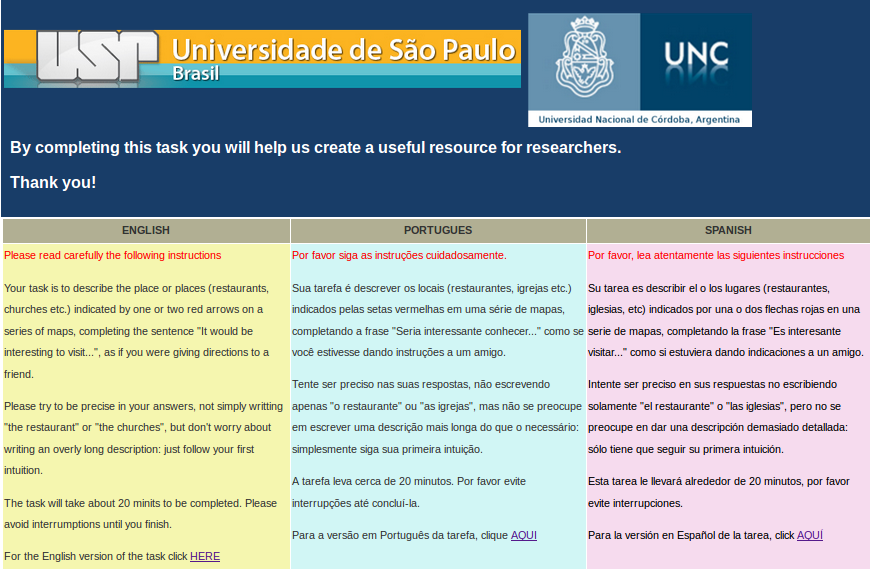
\includegraphics[width=\textwidth]{images/pagPrincipal.png}
\caption{Primera p\'agina del experimento.}
\label{fig-pagPrincipal}
\end{center}
\end{figure}

Una vez seleccionado el idioma del experimento, se solicitaba informaci\'on demogr\'afica de los participantes, como se muestra en la Figura \ref{fig-nacionalidadGenero}. Tambi\'en se solicitaba que se acepten los t\'erminos y condiciones que dec\'ian que los datos ingresados ser\'an usados para investigaci\'on.

\begin{figure}[t]
\begin{center}
\frame{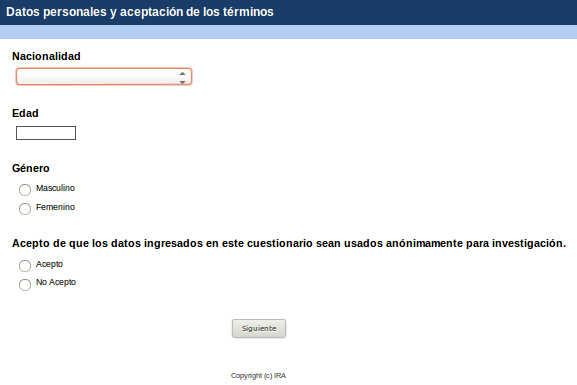
\includegraphics[width=13cm]{images/nacionalidadGenero.png}}
\caption{Datos requeridos.}
\label{fig-nacionalidadGenero}
\end{center}
\end{figure}

En la Figura \ref{fig-interface} se ve una imagen est\'imulo, un mensaje ``Es interesante visitar...'' que es la oraci\'on que el participantente ten\'ia que completar con una expresi\'on referencial del o los objetos apuntados por las flechas. Tambi\'en se ve\'ia una barra indicadora de progreso, y las instrucciones. 

\begin{figure}[h]
\begin{center}
\frame{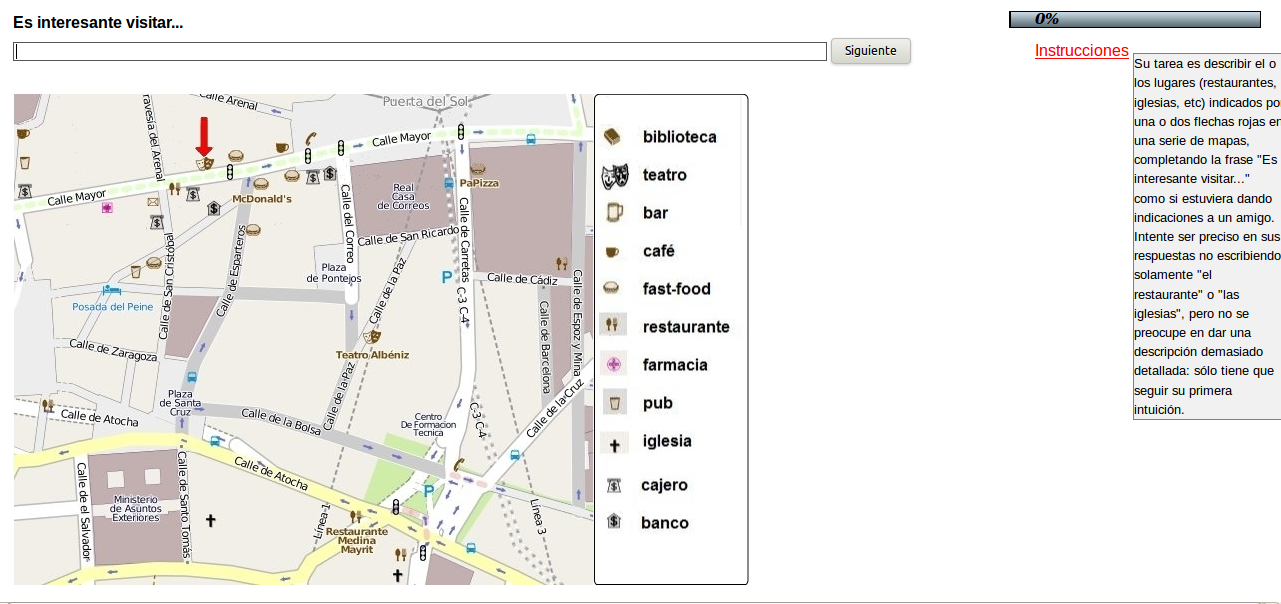
\includegraphics[width=\textwidth]{images/primerImagen.png}}
\caption{Interface del experimento.}
\label{fig-interface}
\end{center}
\end{figure}

\section{Im\'agenes est\'imulo del corpus ZOOM}\label{imagenes-zoom}

Aqu\'i se muestran las im\'agenes que se mostraron a los participantes que completaron la tarea de recolecci\'on del corpus ZOOM para el espa\~nol. El corpus cuenta con im\'agenes sin y con zoom, para targets singulares y plurales.%\footnote{Las im\'agenes muestran fragmentos de mapas de la ciudad de Madrid.}

\subsection{Est\'imulos singulares}

Se muestran mapas con targets singulares. Las im\'agenes (a) muestran targets singleton. La imagen (b) correspondiente muestra el mismo target pero con zoom.

\noindent
\begin{center}
\begin{tabular}{c c}
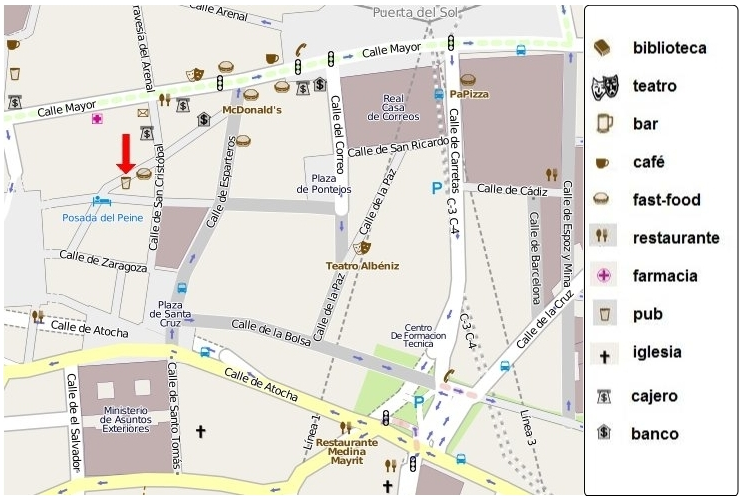
\includegraphics[width=0.46\textwidth]{images/corpus/mapa3.png} & 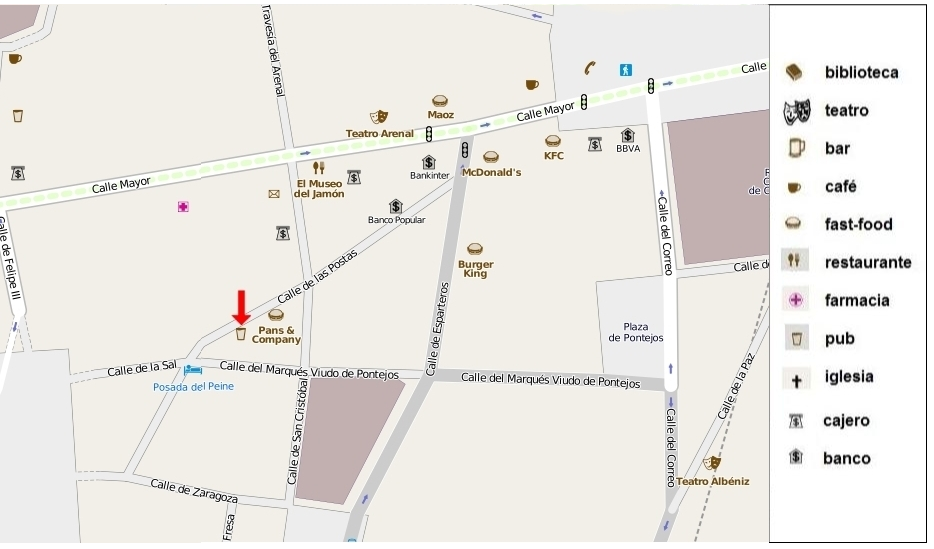
\includegraphics[width=0.53\textwidth]{images/corpus/mapa13.png} \\
(a) & (b) \\
& \\
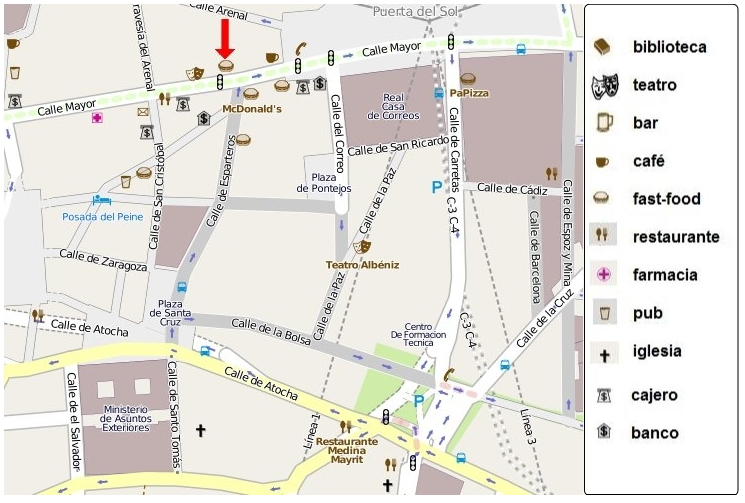
\includegraphics[width=0.46\textwidth]{images/corpus/mapa4.png} & 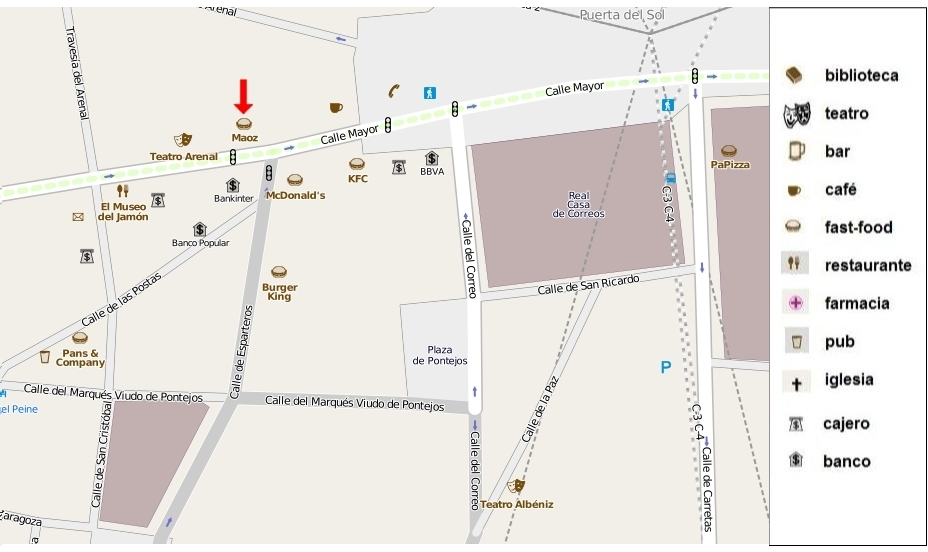
\includegraphics[width=0.53\textwidth]{images/corpus/mapa14.png} \\
(a) & (b) \\
& \\
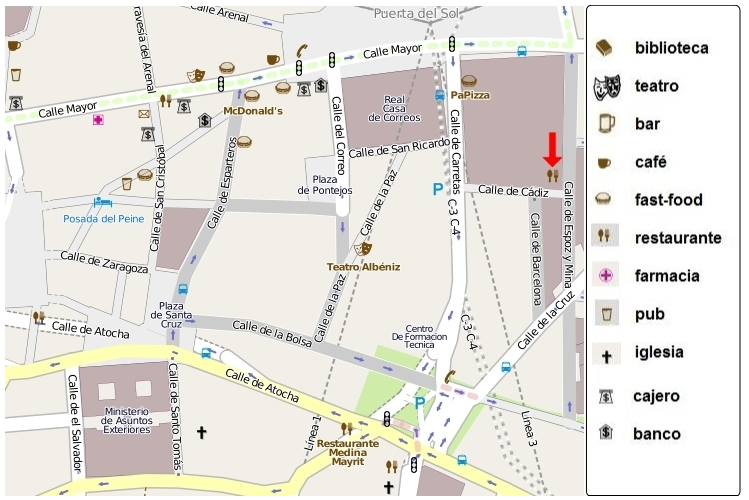
\includegraphics[width=0.46\textwidth]{images/corpus/mapa5.png} & 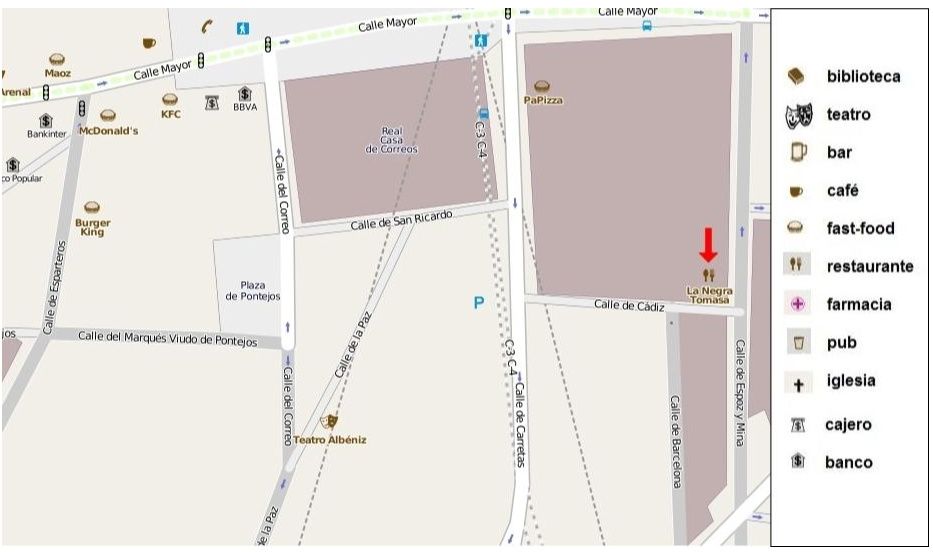
\includegraphics[width=0.53\textwidth]{images/corpus/mapa15.png} \\
(a) & (b) \\
\end{tabular}
\end{center}

\noindent
\begin{center}
\begin{tabular}{c c}
& \\
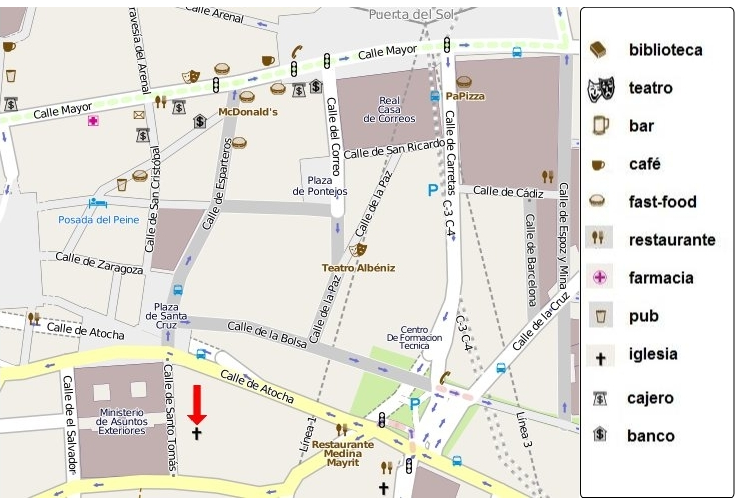
\includegraphics[width=0.46\textwidth]{images/corpus/mapa6.png} & 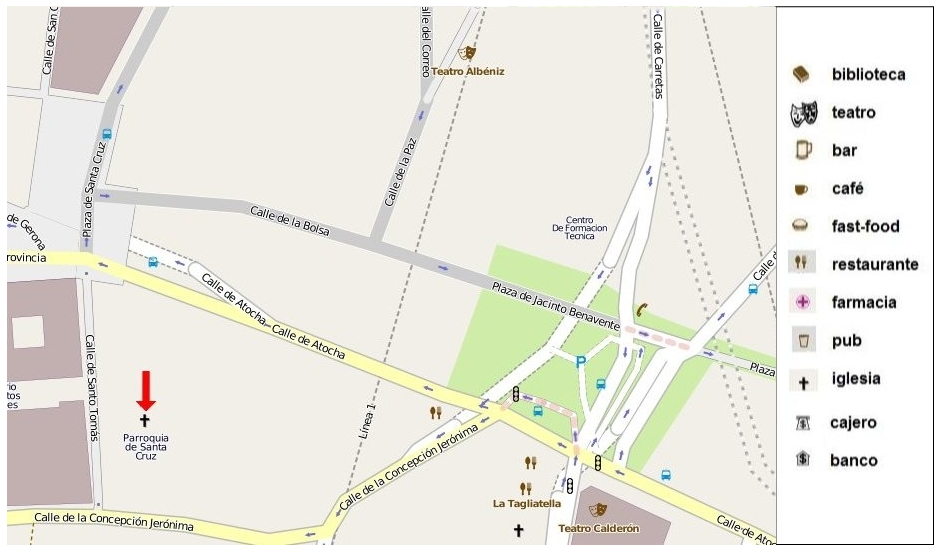
\includegraphics[width=0.53\textwidth]{images/corpus/mapa16.png} \\
(a) & (b) \\
& \\
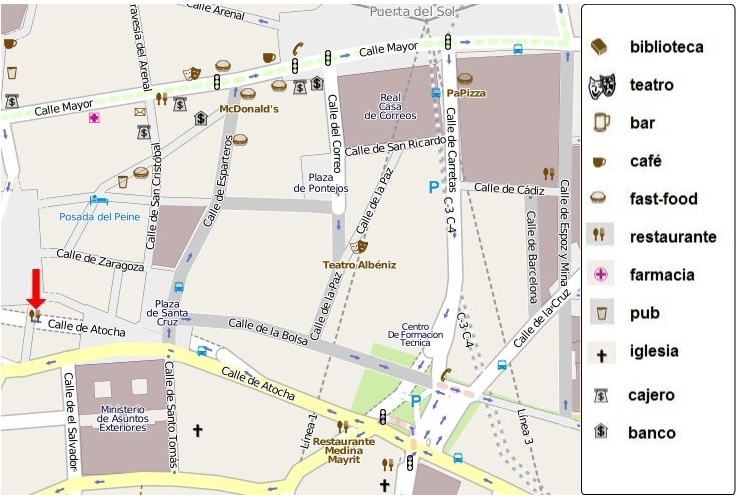
\includegraphics[width=0.46\textwidth]{images/corpus/mapa7.png} & 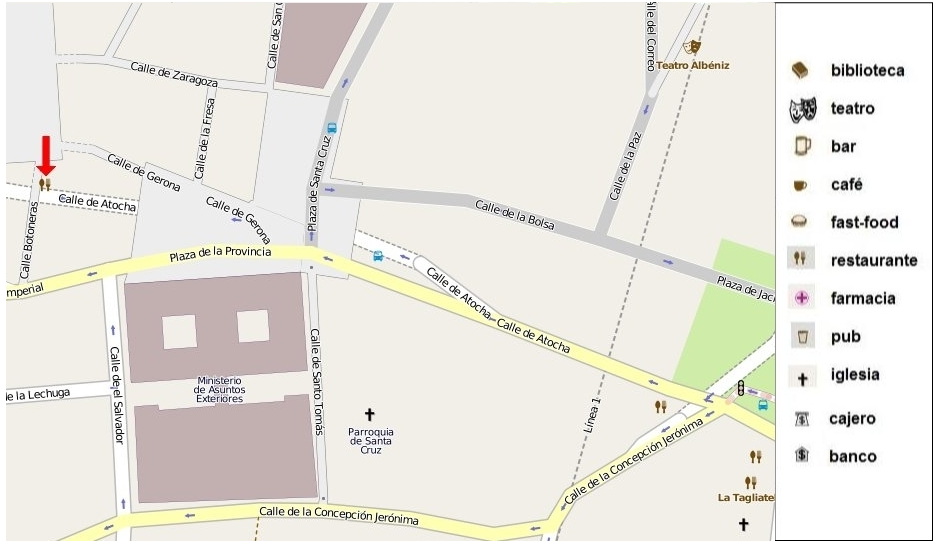
\includegraphics[width=0.53\textwidth]{images/corpus/mapa17.png} \\
(a) & (b) \\
\end{tabular}
\end{center}




\subsection{Est\'imulos plurales}

Se muestran mapas con targets plurales. Las im\'agenes (a) muestran targets con 2 elementos. La imagen (b) correspondiente muestra el mismo target pero con zoom.

\noindent
\begin{center}
\begin{tabular}{c c}
& \\
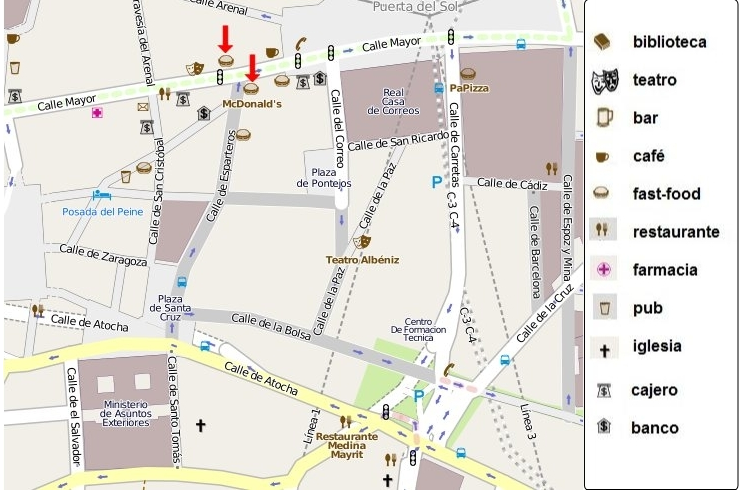
\includegraphics[width=0.46\textwidth]{images/corpus/mapa8.png} & 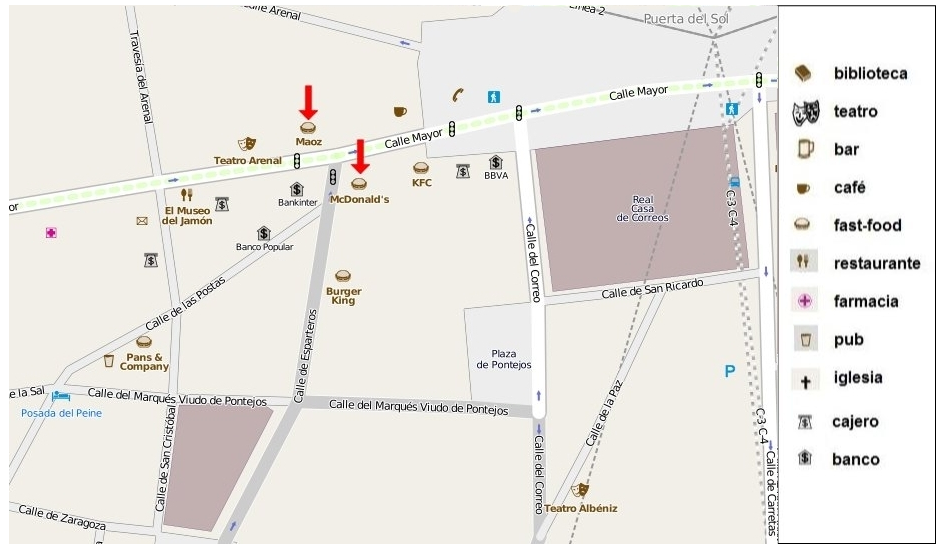
\includegraphics[width=0.53\textwidth]{images/corpus/mapa18.png} \\
(a) & (b) \\
& \\
\end{tabular}
\end{center}

\noindent
\begin{center}
\begin{tabular}{c c}
& \\
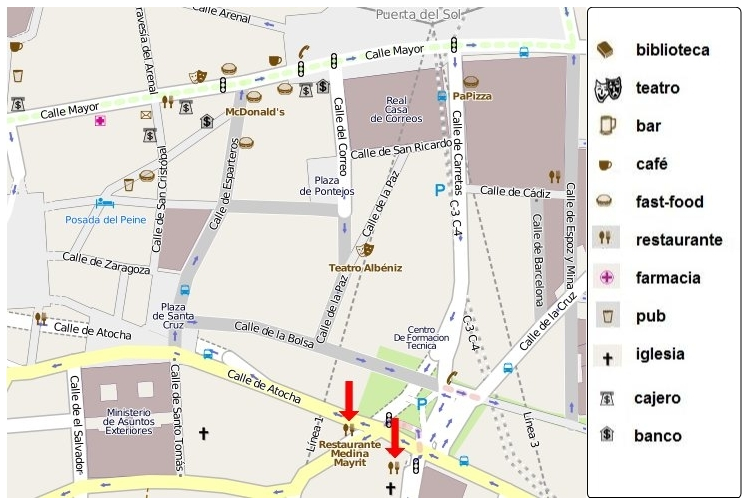
\includegraphics[width=0.46\textwidth]{images/corpus/mapa10.png} & 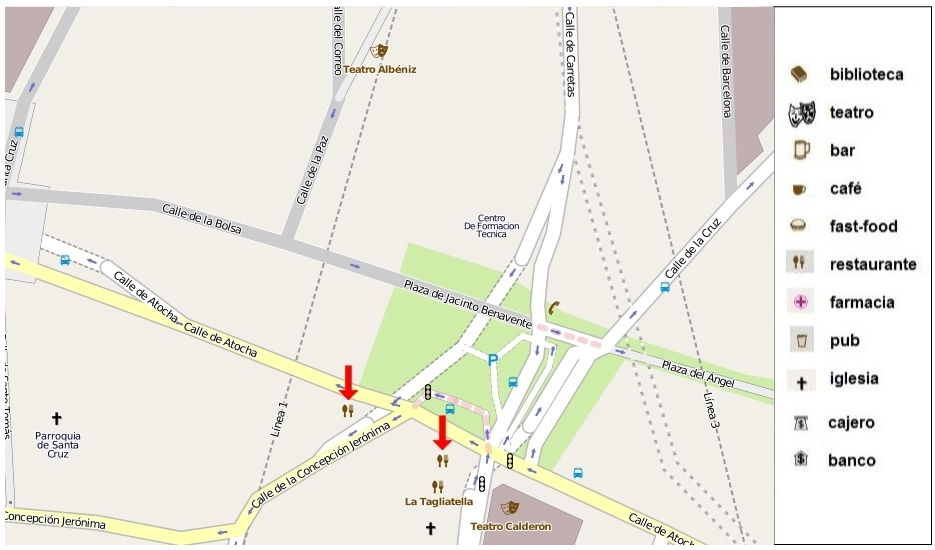
\includegraphics[width=0.53\textwidth]{images/corpus/mapa20.png} \\
(a) & (b) \\
& \\
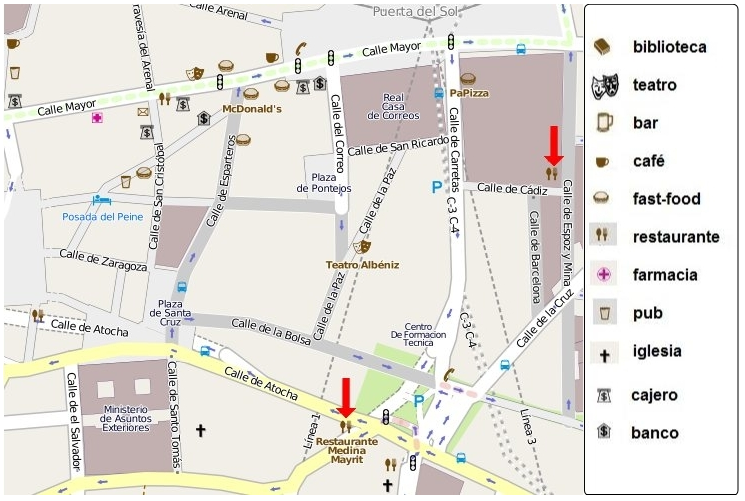
\includegraphics[width=0.46\textwidth]{images/corpus/mapa9.png} & 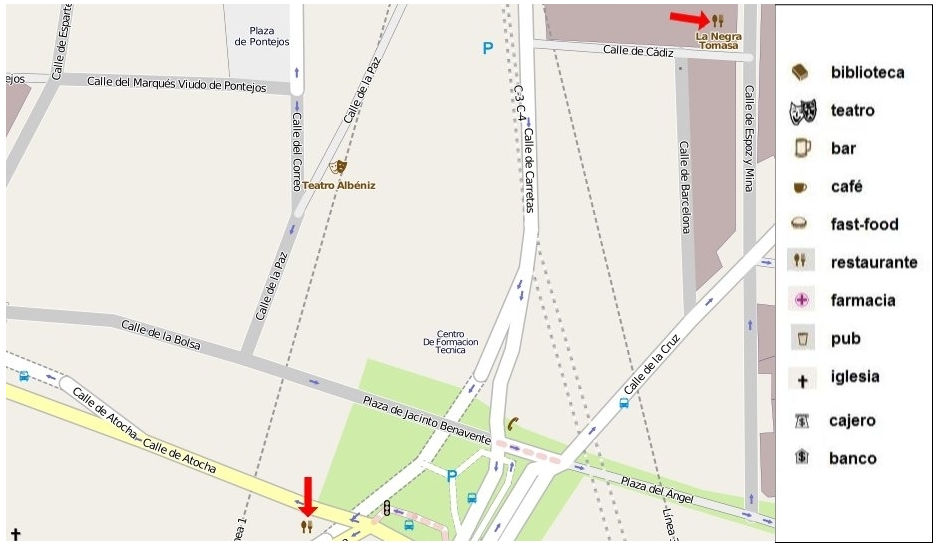
\includegraphics[width=0.53\textwidth]{images/corpus/mapa19.png} \\
(a) & (b) \\
& \\
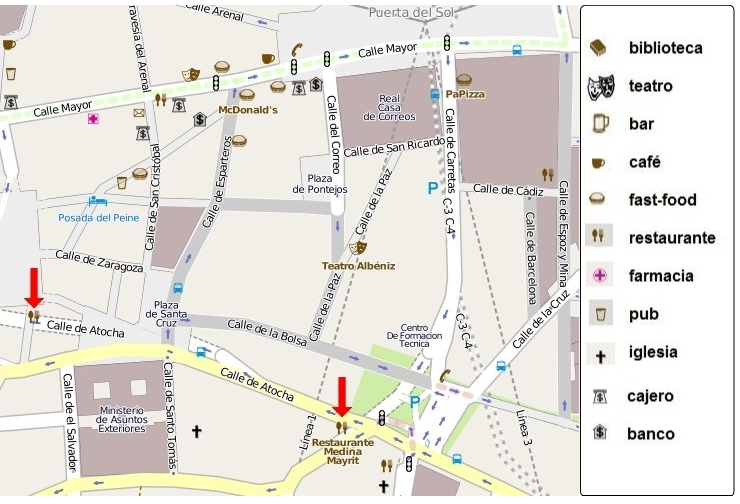
\includegraphics[width=0.46\textwidth]{images/corpus/mapa11.png} & 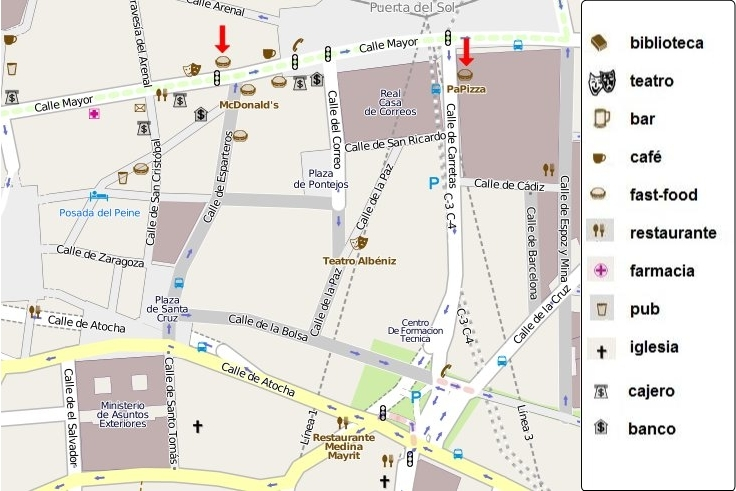
\includegraphics[width=0.53\textwidth]{images/corpus/falta.png} \\
(a) & (b) \\
& \\
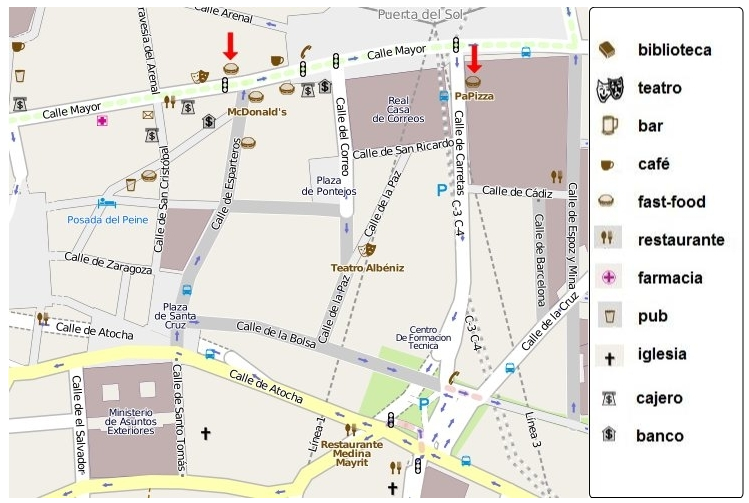
\includegraphics[width=0.46\textwidth]{images/corpus/mapa12.png} & 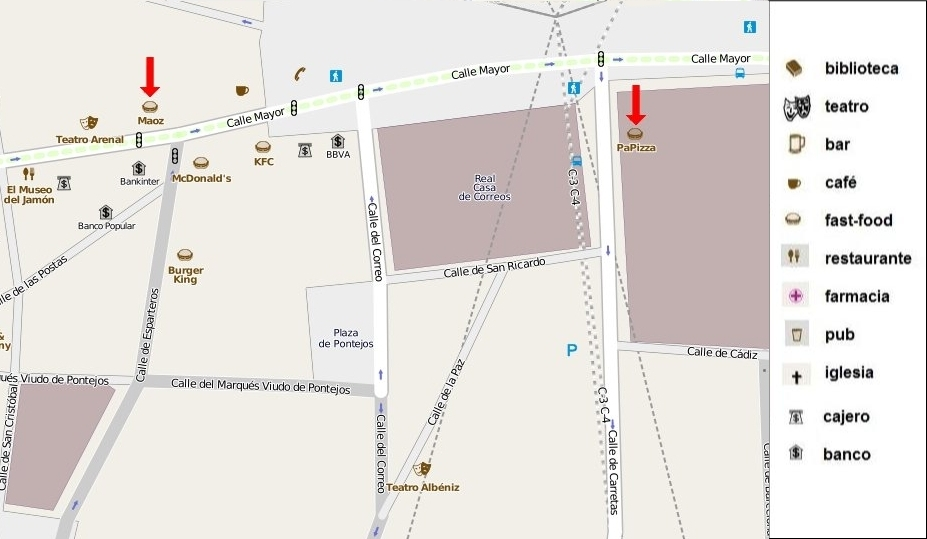
\includegraphics[width=0.53\textwidth]{images/corpus/falta2.png} \\
(a) & (b) \\
\end{tabular}
\end{center}




\clearpage
\section{Modelo relacional que representa un mapa del corpus}

Este modelo relacional representa los casos de estudios de las secciones \ref{sec:conzoom} y \ref{sec:plural} y representan el mapa de la Figura \ref{mapa-zoom2x}.

\vspace*{2cm}
\begin{figure}[h]
\centering
\begin{tikzpicture}
  [
    n/.style={circle,draw,inner sep=3pt,node distance=4cm},
    aArrow/.style={->, >=stealth, thick, shorten <= 1pt, shorten >= 1pt},	
  ]
	\node[n,label=below:{
    \relsize{-2}$\begin{array}{c}
     \nStreet\end{array}$}] (a) {\relsize{-2}$str17$};		
	 \node[n,label=above:{
    \relsize{-2}$\begin{array}{c}
      \nBuilding\end{array}$}, above of=a] (f) {\relsize{-2}$min1$};	
					 
	\node[n,label=above:{
    \relsize{-2}$\begin{array}{c}
		 \nChurch\\[-3pt] 
     \nParroquiaDeSantaCruz\end{array}$}, above of=f] (g) {\relsize{-2}$church1$};
	\node[n,label=above:{
    \relsize{-2}$\begin{array}{c}
      \nStreet\\[-3pt] 
      \nCalleDeLaConcepcionJeronima\end{array}$}, above of=g] (z) {\relsize{-2}$str22$};
			
	\node[n,label=above:{
    \relsize{-2}$\begin{array}{c}
      \nStreet\end{array}$}, right of=z] (y) {\relsize{-2}$str25$};	
				
	\node[n,label=below:{
    \relsize{-2}$\begin{array}{c}
      \nStreet\\[-3pt] 
      \nCalleDeElSalvador\end{array}$}, right of=a] (b) {\relsize{-2}$str12$};
   
	\node[n,label=below:{
    \relsize{-2}$\begin{array}{c}
      \nStreet\end{array}$}, right of=b] (m) {\relsize{-2}$str16$};		 

  \node[n,label=above:{
    \relsize{-2}$\begin{array}{c}
      \nStreet\\[-3pt] 
      \nCalleSantoTomas\end{array}$}, above of=b] (c) {\relsize{-2}$str10$};	
			
  \node[n,label=below:{
    \relsize{-2}$\begin{array}{c}
     \nChurch\end{array}$}, right of=c] (d) {\relsize{-2}$church2$};
			
  \node[n,label=above:{
    \relsize{-2}$\begin{array}{c}
      \nRestaurante\end{array}$}, above of=d] (h) {\relsize{-2}$rest3$};			
			
  \node[n,label=above:{
    \relsize{-2}$\begin{array}{c}
      \nStreet\\[-3pt] 
      \nCalleAtocha\end{array}$}, above of=c] (e) {\relsize{-2}$str9$};		

  \node[n,label=right:{
    \relsize{-2}$\begin{array}{c}
      \nRestaurante\\[-3pt] 
      \nLaTagliatella\end{array}$}, right of=m] (k) {\relsize{-2}$rest4$};

 \node[n,label=below:{
    \relsize{-2}$\begin{array}{c}
      \nRestaurante\end{array}$}, below of=k] (w) {\relsize{-2}$rest5$};

  \node[n,label=below:{
    \relsize{-2}$\begin{array}{c}
      \nTeatroCalderon\end{array}$}, right of=d] (i) {\relsize{-2}$thea0$};
		
  \node[n,label=above:{
    \relsize{-2}$\begin{array}{c}
      \nStreet\\[-3pt] 
      \nCalleDeCarretas\end{array}$}, right of=h] (x) {\relsize{-2}$str15$};	

%\node[n,label=below:$str17\nStreet$,label=above:{
 %   \relsize{-2}}, below of=k] (n) {};				
 \draw [aArrow,<->,bend right=40] (g) to node[auto,swap]{\relsize{-2}$\nFrenteCerca$} (f);
% \draw [aArrow,bend right=40] (f) to node[auto,swap]{\relsize{-2}$\nFrenteCerca$} (g);

 \draw [aArrow,bend right=40] (g) to node[auto,swap]{\relsize{-2}$\nIn$} (c);
 \draw [aArrow,bend right=20] (g) to node[auto,swap]{\relsize{-2}$\nIn$} (z);
 \draw [aArrow,bend right=20] (g) to node[auto,swap]{\relsize{-2}$\nIn$} (y);
 \draw [aArrow,bend right=40] (d) to node[auto,swap]{\relsize{-2}$\nIn$} (m);
 \draw [aArrow,<->,bend right=-20] (d) to node[auto,swap]{\relsize{-2}$\nFrenteCerca$} (i);
 %\draw [aArrow,bend right=40] (i) to node[auto,swap]{\relsize{-2}$\nFrente$} (d);
 \draw [aArrow,<->,bend right=-20] (k) to node[auto,swap]{\relsize{-2}$\nCerca$} (d);
 \draw [aArrow,<->,bend right=40] (k) to node[auto,swap]{\relsize{-2}$\nCerca$} (w);
 %\draw [aArrow,bend right=40] (d) to node[auto,swap]{\relsize{-2}$\nCerca$} (k);
 \draw [aArrow,<->,bend right=40] (k) to node[auto,swap]{\relsize{-2}$\nIn$} (x);
 \draw [aArrow,bend right=40] (k) to node[auto,swap]{\relsize{-2}$\nIn$} (m);
 \draw [aArrow,<->,bend right=40] (k) to node[auto,swap]{\relsize{-2}$\nFrenteCerca$} (i);
% \draw [aArrow,bend right=40] (i) to node[auto,swap]{\relsize{-2}$\nFrente$} (k);
 \draw [aArrow,bend right=20] (h) to node[auto,swap]{\relsize{-2}$\nIn$} (e);
 \draw [aArrow,bend right=20] (h) to node[auto,swap]{\relsize{-2}$\nIn$} (j);

 \draw [aArrow,bend right=30] (f) to node[auto,swap]{\relsize{-2}$\nIn$} (c);
 \draw [aArrow,bend right=40] (f) to node[auto,swap]{\relsize{-2}$\nIn$} (e);
 \draw [aArrow,bend right=40] (f) to node[auto,swap]{\relsize{-2}$\nIn$} (a);
 \draw [aArrow,bend right=40] (f) to node[auto,swap]{\relsize{-2}$\nIn$} (b); 

 \draw [aArrow,bend right=5] (i) to node[auto,swap]{\relsize{-2}$\nIn$} (e);
 \draw [aArrow,bend right=40] (i) to node[auto,swap]{\relsize{-2}$\nIn$} (m);

 \end{tikzpicture}
\caption{Modelo relacional del mapa de la Figura \ref{mapa-zoom2x}.}
\label{modelo-mapa-zoom2x}
\end{figure}


\chapter{F\'ormulas generadas por nuestro algoritmo}\label{apendiceB}

En este ap\'endice mostramos f\'ormulas que representan expresiones referenciales generadas usando el algoritmo presentado en el Cap\'itulo \ref{sec:algoritmo} para los corpora GRE3D7 y ZOOM. 

\section{Generaci\'on sobre el corpus GRE3D7}

En esta secci\'on mostramos f\'ormulas que representan expresiones referenciales para los est\'imulos del corpus GRE3D7 generadas usando el algoritmo presentado en el Cap\'itulo \ref{sec:algoritmo}. Tambie\'en mostramos las im\'agenes est\'imulo del corpus que usamos en esta tesis para la evaluaci\'on presentada en el Cap\'itulo \ref{sec:evaluacion}. 

\subsection{Ejemplos de f\'ormulas}
\label{formulas-gre3d7}

En la Secci\'on \ref{sec:ejemplo_ejecucion} se mostr\'o un ejemplo de ejecuci\'on del algoritmo para la Figura \ref{GRE3D7-stimulus1-ids}, aqu\'i mostramos todas las f\'ormulas que di\'o el algoritmo para el target se\~nalado por la flecha, en 10000 ejecuciones.


\begin{table}[h]
\begin{center}
\begin{tabular}{|l|l|c|}
\hline
&F\'ormula			      &  \# \\ \hline \hline

1&$\exists \nBall \land \exists \nLarge \land \exists \aRed$		&6003 \\ \hline
2&$\exists \nBall \land \exists \aRed$		&3672 \\ \hline
3&$\exists \nBall \land \exists \nLarge$		&53 \\ \hline
4&$\exists \nBall \land \exists \aRed \land \exists \nRightof$	&	248 \\ \hline
5&$\exists \nBall \land \exists \nRightof$		&15 \\ \hline
6&$\exists \nBall \land \exists \nRightof(\exists \nCube)$	&	7 \\ \hline
7&$\exists \nBall \land \exists \nRightof(\exists \nCube \land \exists \nLarge)$&		1 \\ \hline
8&$\exists \nBall \land \exists \nRightof(\exists \nCube \land \exists \aRed)$		&1 \\ \hline

\end{tabular}

\caption{F\'ormulas dadas por el algoritmo para el modelo de la Figura \protect\ref{fig4-9}.}\label{formulas-mapa-gre3d7-apendice}
\end{center}
\end{table}

\subsection{Im\'agenes verde-azules del corpus}
\label{imagenesGRE3D7-apendice}
En la Figura \ref{verde-azul} se muestran las escenas mostradas a los participantes del corpus \textit{GRE3D7} introducido en la Secci\'on \ref{sec:corpusGRE}, esta parte incluye s\'olo las escenas verde y azules. El corpus contiene otra parte similar con colores rojo y amarillo.

\begin{figure}[h]
\centering
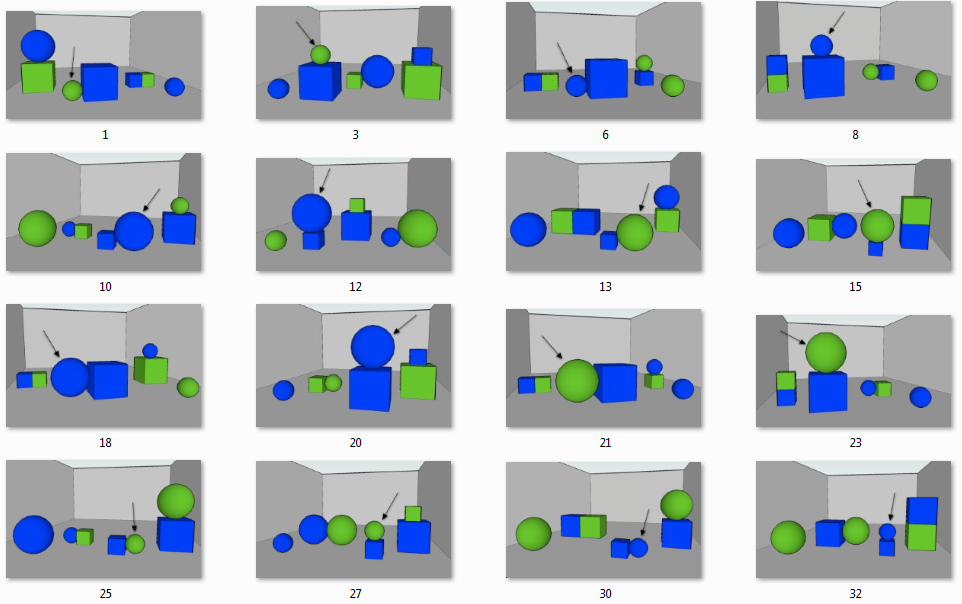
\includegraphics[width=1\textwidth]{images/corpusVerdeAzul.png}
\caption{Im\'agenes del \textit{GRE3D7} parte azul y verde.}
\label{verde-azul}
\end{figure}


\section{ERs dadas por el algoritmo para corpus ZOOM} \label{er-mapa-zoom}

En la Tabla \ref{formulas-mapa-zoom2x-apendice} se muestran las f\'ormulas generadas por el algoritmo para el caso de estudio mostrado en la Secci\'on \ref{sec:conzoom}, ejecutando el algoritmo 1000 veces.

\begin{table}[h]
\begin{center}
\begin{tabular}{|l|l|c|}
\hline
&F\'ormula                           &  \# \\ \hline \hline
1& $\exists \nParroquiaDeSantaCruz$& 570\\ \hline

2& $\exists \nParroquiaDeSantaCruz. \exists \nIn(T)$& 174\\ \hline
3& $\exists \nParroquiaDeSantaCruz. \exists \nIn(\exists \nCalleSantoTomas)$& 72\\ \hline
4& $\exists \nParroquiaDeSantaCruz. \land \exists.\nCerca(T)$& 57\\ \hline

5& $\exists \nChurch \land \exists \nParroquiaDeSantaCruz$& 48\\ \hline
6& $\exists \nChurch \land \exists \nParroquiaDeSantaCruz. \exists \nIn(T)$& 17\\ \hline
7& $\exists \nParroquiaDeSantaCruz \land \exists. \nIn(\exists \nCalleConJer)$& 13\\ \hline
8& $\exists \nChurch \land \land \exists. \nIn(\exists \nCalleConJer) $&10\\ \hline

9& $\exists \nIn(\exists \nCalleSantoTomas) \land \exists \nChurch$&9\\ \hline

10& $\exists \nChurch \land \exists \nIn(\exists \nCalleSantoTomas))$&7\\ \hline


\end{tabular}

\caption{F\'ormulas dadas por el algoritmo para el modelo de la Figura \protect\ref{modelo-mapa-zoom2x}.}\label{formulas-mapa-zoom2x-apendice}
\end{center}
\end{table}


Las f\'ormulas mostradas en la Tabla \ref{formulas-mapa-zoom-ap}, fueron generadas por el algoritmo en el caso de estudio presentado en la Secci\'on \ref{sec:sinzoom}. Ejecutando el algoritmo 1000 veces.

\begin{table}[h]
\begin{center}
\begin{tabular}{|l|l|c|}
\hline
&F\'ormula			      &  \# \\ \hline \hline

1&$\exists \nChurch.(T) \land \exists \nIn .(\exists \nCalleSantoTomas))$ &234 \\ \hline

2&$\exists \nFront . (\exists \nMinAsExt)$ &202 \\ \hline

3&$\exists \nChurch.(T) \land \exists \nIn .(\exists \nCalleAtocha)$ &87\\ \hline

4&$\exists \nNear .(\exists \nMinAsExt .(T))$ &79\\ \hline

5&$\exists \nFront.(\exists \nFront.(\exists \nChurch.(T))) \land \exists \nIn .(\exists \nCalleSantoTomas))$ &74\\ \hline

6&$\exists \nChurch.(T) \land \exists\nFront . (\exists \nMinAsExt))$ &71\\ \hline

7&$\exists \nChurch.(T) \land \exists\nFront . (\exists \nMinAsExt) \land \exists \nIn .(T))$ &65\\ \hline

8&$\exists \nFront.(\exists \nIn .(\exists \nCalleSantoTomas))) \land \exists \nChurch.(T) \land \exists \nIn .(T)$ &53\\ \hline

9&$\exists \nFront . (\exists \nMinAsExt) \land \exists \nIn .(T))$ &21\\ \hline

10&$\exists \nNear .(\exists \nMinAsExt .(T) \land \exists \nIn .(T))$ &15\\ \hline

11&$\exists  \nNear.(\exists \nIn .(\exists \nCalleSantoTomas))) \land \exists \nChurch.(T)$ &13\\ \hline

12&$\exists  \nNear.(\exists \nFront.(\exists \nChurch.(T))) \land \exists \nIn .(\exists \nCalleAtocha)$ &11\\ \hline

13&$\exists \nFront.(\exists \nIn .(\exists \nCalleSantoTomas))) \land \exists \nChurch.(T)$ &11\\ \hline

14&$\exists \nChurch.(T) \land \exists \nIn .(\exists \nCalleAtocha) \land \exists \nFront.(\exists \nFront.(\exists \nChurch.(T)))$ &10\\ \hline

15&$\exists  \nNear.(\exists \nNear.(\exists \nChurch.(T))) \land \exists \nIn .(\exists \nCalleSantoTomas))$ &8\\ \hline

16&$\exists  \nNear.(\exists \nIn .(\exists \nCalleSantoTomas))) \land \exists \nChurch.(T) \land \exists \nIn .(T)$ &6\\ \hline

17&$\exists \nChurch.(T) \land \exists \nNear .(\exists \nMinAsExt .(T) \land \exists \nIn .(T))$ &6\\ \hline

18&$\exists  \nNear.(\exists \nNear.(\exists \nChurch.(T) \land \exists \nIn .(T))) \land \exists \nIn .(\exists \nCalleSantoTomas))$ &5\\ \hline

19&$\exists \nFront.(\exists \nFront.(\exists \nChurch.(T) \land \exists \nIn .(T))) \land \exists \nIn .(\exists \nCalleSantoTomas))$ &5\\ \hline

20&$\exists  \nIn .(\exists \nCalleSantoTomas)) \land \exists \nChurch.(T)$ &4\\ \hline

21&$\exists \nChurch.(T) \land \exists \nNear .(\exists \nMinAsExt .(T))$ &4\\ \hline

22&$\exists  \nNear.(\exists \nFront.(\exists \nChurch.(T))) \land \exists \nIn .(\exists \nCalleSantoTomas))$ &4\\ \hline

23&$\exists \nFront.(\exists \nNear.(\exists \nChurch.(T))) \land \exists \nIn .(\exists \nCalleSantoTomas))$ &3\\ \hline

24&$\exists \nChurch.(T) \land \exists \nNear.(\exists \nNear.(\exists \nChurch.(T))) \land \exists \nIn .(\exists \nCalleAtocha)$ &2\\ \hline

25&$\exists  \nNear.(\exists \nFront.(\exists \nChurch.(T) \land \exists \nIn .(T))) \land \exists \nIn .(\exists \nCalleAtocha)$ &2\\ \hline

26&$\exists \nChurch.(T) \land \exists \nIn .(\exists \nCalleAtocha) \land \exists \nNear.(\exists \nNear.(\exists \nChurch.(T)))$ &2\\ \hline

27&$\exists \nFront.(\exists \nIn .(\exists \nCalleSantoTomas))) \land \exists \nNear.(\exists \nNear.(\exists \nChurch.(T)))$ &1\\ \hline

28&$\exists \nFront . (\exists \nMinAsExt) \land \exists \nIn .(\exists \nCalleAtocha))$ &1\\ \hline

29&$\exists  \nIn .(\exists \nCalleAtocha) \land \exists \nChurch.(T)$ &1\\ \hline

\end{tabular}

\caption{F\'ormulas dadas por el algoritmo para el modelo de la Figura \protect\ref{modelo-mapa-zoom}.}\label{formulas-mapa-zoom-ap}
\end{center}
\end{table}



En la Tabla \ref{formulas-mapa-zoom2-apendice} se muestran las f\'ormulas dadas por el algoritmo en 1000 ejecuciones para la Figura \ref{mapa-zoom-plural}, mostrado en la Secci\'on \ref{sec:plural}, ejecutando el algoritmo 1000 veces. 

\label{formulas-plurales}
\begin{table}[h]
\begin{center}
\begin{tabular}{|l|l|c|}
\hline
&F\'ormula			      &  \# \\ \hline \hline

1&$rest_3 = \exists \nMedinaMayrit$ &303\\
 &$rest_4 = \exists \nNear.(\exists \nMedinaMayrit)$& \\ \hline

2&$rest_3 = \exists \nMedinaMayrit$ & 285\\  
 &$rest_4 =  \exists \nNear. (\exists \nNear.(\exists \nMedinaMayrit)) \land \exists \nNear.(\exists \nMedinaMayrit)$& \\ \hline

3&$rest_3 =\exists \nMedinaMayrit \land \exists \nIn.(T)$ & 105\\ 
 &$rest_4 =\exists \nNear.(\exists \nMedinaMayrit \land \exists \nIn.(T))$& \\ \hline

4&$rest_3 =\exists \nMedinaMayrit \land \exists \nIn.(\exists \nCalleAtocha)$ &83 \\ 
 &$rest_4 =\exists \nNear.(\exists \nMedinaMayrit  \land \exists \nIn.(\exists \nCalleAtocha))$& \\ \hline

5&$rest_3 =\exists \nMedinaMayrit  \land \exists \nIn.(\exists \nCalleAtocha)$&77 \\ 
 &$\land \exists \nNear.(\exists \nNear.(\exists \nMedinaMayrit))$& \\
&$rest_4 = \exists \nNear.(\exists \nMedinaMayrit)$& \\ \hline

6&$rest_3 =\exists \nNear.(\exists \nIn.(\exists \nCalleDeLaCruz))  \land \exists \nIn.(\exists \nCalleDeCarretas) \land $ & 20\\
&$\exists \nIn.(\exists \nCalleDeLaCruz)  \land \exists \nNear.(\exists \nIn.(\exists \nCalleDeCarretas))$& \\ \hline

7&$rest_3 =\exists \nMedinaMayrit  $&13 \\ 
&$\land \exists \nNear.(\exists \nIn.(\exists \nCalleDeLaCruz))  \land \exists \nIn.(\exists \nCalleAtocha)$ & \\
&$rest_4 = \exists \nNear.(\exists \nMedinaMayrit)$&\\ \hline

8&$rest_3 =\exists \nIn.(\exists \nCalleDeCarretas)  \land \exists \nNear.(\exists \nNear.$&9\\
&$(\exists \nNear.(\exists \nNear.(\exists$ &\\
&$\nNear.(\exists \nIn.(\exists \nCalleDeCarretas)))))) $&\\
&$rest_4 = \exists \nNear.(\exists \nIn.(\exists \nCalleDeCarretas)  $ & \\
&$\land \exists \nNear.(\exists \nNear.(\exists \nNear.(\exists \nNear.(\exists \nNear.$&\\
&$(\exists \nIn.(\exists \nCalleDeCarretas)))))))$&\\ \hline

9&$rest_3 =\exists \nMedinaMayrit \land \exists \nIn.(\exists \nCalleAtocha)$ & 9\\
&$rest_4 = \exists \nNear.(\exists \nIn.(\exists \nCalleAtocha) $ & \\
&$ \land \exists \nNear.(\exists \nNear.(\exists \nChurch.(T)  \land \exists \nNear.(\exists \nIn.(\exists \nCalleAtocha)  $ & \\
&$\land \exists \nNear.(\exists \nNear.(\exists \nChurch.(T)  \land \exists \nIn.(T)))))))$&\\ \hline

10&$rest_3 = \exists \nNear.(\exists \nIn.(\exists \nCalleAtocha)  \land \exists \nNear.(\exists \nNear.(\exists \nIn.(\exists \nCalleAtocha) $ & 9\\
&$ \land \exists \nNear.(\exists \nNear.(\exists \nIn.(\exists \nCalleDeCarretas))))))  \land \exists \nIn.(\exists \nCalleDeCarretas)  $ & \\
&$rest_4 = \exists \nNear.(\exists \nNear.(\exists \nIn.(\exists \nCalleAtocha)  \land \exists \nNear.(\exists \nNear.$ & \\
&$(\exists \nIn.(\exists \nCalleAtocha)  \land \exists \nNear.(\exists \nNear.(\exists \nIn.(\exists \nCalleDeCarretas)))))) $ & \\
&$ \land \exists \nIn.(\exists \nCalleDeCarretas))$&\\ \hline

\end{tabular}

\caption{Las 10 f\'ormulas m\'as frecuentes dadas por el algoritmo para el modelo de la Figura \protect\ref{modelo-mapa-zoom}. Tomando como target 2 restaurantes.}\label{formulas-mapa-zoom2-apendice}
\end{center}
\end{table}


